\documentclass[titlepage]{jarticle}
\usepackage{h31ec-exp}
\usepackage[dvipdfmx]{graphicx}
\usepackage{here}

\title{オームの法則の実験}
\grade{1年39番}%
\author{鷲尾 優作}
\team{}
\date{令和元年7月16日}
\expdate{令和元年7月9日}
\coauthor{%
  23番 & 高橋 匠\\
  24番 & 高橋 尚也\\
  31番 & 羽田 伊吹}

\begin{document}
\maketitle

\section{本実験の目的}
オームの法則を実験することにより、確認し、その応用ができるようにする。

\section{理論}
電気抵抗に流れる電流は、これに加えた電圧に比例し、抵抗に逆比例する。\\
この法則はあるゆる電気理論の基礎となるもので、A・V・Ωの単位を用いることで、\\
比例定数は1となり、以下の簡単な式で表すことができる。
\begin{equation}
    I[A]=V[V]/R[Ω]
\end{equation}
\begin{equation}
    V[V]=R[Ω]*I[A]
\end{equation}
\begin{equation}
    R[Ω]=V[V]/I[A]
\end{equation}

\section{実験内容}
\subsection{[実験1]抵抗電流特性}
\subsubsection{手順1 回路の作成}
\begin{figure}[H]
    \begin{center}
        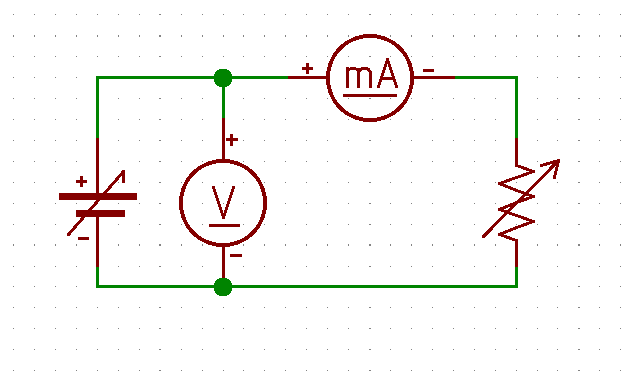
\includegraphics[width=8cm]{04.png}
        \caption{抵抗電流特性測定回路}
    \end{center}
\end{figure}
第1図のような回路を作成する。
\subsubsection{手順2 電圧の固定}
電圧を5,7,10Vのいずれかに固定する。なお、それぞれの場合について実験する。
\subsubsection{手順3 可変標準抵抗の操作及び記録}
可変標準抵抗(負荷抵抗)R[Ω]を0.1-1KΩまで0.1KΩ毎に増加させる。\\
その都度、電流計の電流値を読み記録する。
\subsubsection{手順4 理論値の計算}
2章で示された(1)式に電圧値及び負荷抵抗値を代入し
オームの法則による実験の理論値を求める。\\
この実験での電流値の理論値を求める。

\subsection{[実験2]電圧電流特性}
\subsubsection{手順1 抵抗値の固定}
第1図の回路において、抵抗値を125,250,500Ωのいずれかに固定する。\\
なお、それぞれの場合について実験する。
\subsubsection{手順2 電圧の操作及び記録}
電圧[V]を0-14Vまで1V毎に増加させる。\\
その都度、電流計の電流値を読み記録する。
\subsubsection{手順3 理論値の計算}
2章で示された(1)式に負荷抵抗値及び電圧値を代入し\\
この実験での電流値の理論値を求める。

\section{使用器具}
\begin{enumerate}
    \item 直流電源\\商品名KIKUTU PMC18-3\\定格 INPUT AC100V 50/60Hz Max 230VA\\物品番号Ec-09
    \item 抵抗器\\商品名YAMABAYASHI ELECTRIC CO.,LTD. DECADE RESISTER TYPE YRH-4BA\\
    定格 100Ω 70mAMax, 10Ω 250mAMax, 1Ω 350mAMax, 0.1Ω 550mAMax\\物品番号不明
    \item 電圧計\\商品名YOKOGAWA MODEL2011 CLASS0.5 B9000EU\\定格 0-100V 1000Ω/V\\
    物品番号1-63
    \item 電流計\\商品名YOKOGAWA SYC2021 MODEL205103\\定格 0-1000mA\\物品番号不明
\end{enumerate}

\section{実験結果}
\subsection{[実験1]抵抗電流特性}

\begin{table}[H]
    \centering
    \label{tab:tab`le1}
    \caption{計測結果}
    \begin{tabular}{c|c|c|c|c|c|c|c} \hline \hline
        \multicolumn{2}{c|}{負荷抵抗} & \multicolumn{2}{c|}{5V 電流値I[mA]} 
        & \multicolumn{2}{c|}{7V 電流値I[mA]} & \multicolumn{2}{c}{10V 電流値I[mA]}\\\cline{3-8}
        \multicolumn{2}{c|}{R[kΩ]} & 理論値 & 実測値 & 理論値 & 実測値 & 理論値 & 実測値\\
    \hline
        \multicolumn{2}{c|}{0.1} & 50 & 50.0 & 70 & 70.0 & 100 & 100.0 \\\hline
        \multicolumn{2}{c|}{0.2} & 20 & 25.00 & 35 & 35.0 & 50 & 50.0 \\\hline
        \multicolumn{2}{c|}{0.3} & 17 & 17.00 & 23 & 22.00 & 33 & 33.0 \\ \hline
        \multicolumn{2}{c|}{0.4} & 13 & 12.50 & 18 & 17.50 & 25 & 25.00 \\ \hline
        \multicolumn{2}{c|}{0.5} & 10 & 10.00 & 14 & 14.00 & 20 & 20.25 \\ \hline
        \multicolumn{2}{c|}{0.6} & 8.3 & 8.50 & 12 & 11.75 & 17 & 16.75 \\ \hline
        \multicolumn{2}{c|}{0.7} & 7.1 & 7.00 & 10 & 10.00 & 14 & 14.50 \\ \hline
        \multicolumn{2}{c|}{0.8} & 6.3 & 6.25 & 8.8 & 8.75 & 13 & 12.50 \\ \hline
        \multicolumn{2}{c|}{0.9} & 5.6 & 5.60 & 7.8 & 7.75 & 11 & 11.00 \\ \hline
        \multicolumn{2}{c|}{1.0} & 5.0 & 5.00 & 7.0 & 7.00 & 10 & 10.00 \\ \hline
      \end{tabular}
\end{table}

\begin{figure}[H]
    \begin{center}
        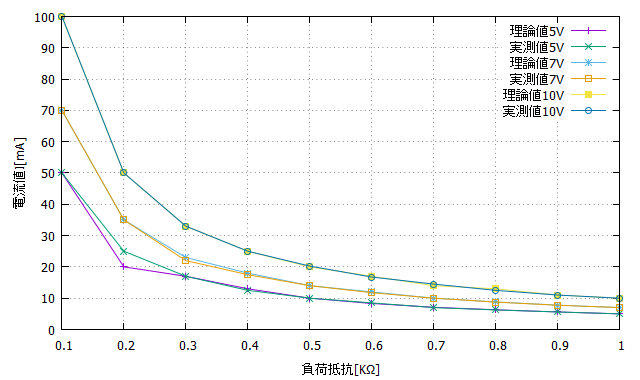
\includegraphics[width=10cm]{01.png}
        \caption{抵抗電流特性グラフ}
    \end{center}
\end{figure}

\subsection{[実験2]電圧電流特性}
\begin{table}[H]
    \centering
    \label{tab:tab`le1}
    \caption{計測結果}
    \begin{tabular}{c|c|c|c|c|c|c|c} \hline \hline
        \multicolumn{2}{c|}{設定電圧} & \multicolumn{2}{c|}{125Ω 電流値I[mA]} 
        & \multicolumn{2}{c|}{250Ω 電流値I[mA]} & \multicolumn{2}{c}{500Ω 電流値I[mA]}\\\cline{3-8}
        \multicolumn{2}{c|}{V[V]} & 理論値 & 実測値 & 理論値 & 実測値 & 理論値 & 実測値\\
    \hline
        \multicolumn{2}{c|}{0} & 0 & 0.00 & 0 & 0.00 & 0 & 0.00 \\\hline
        \multicolumn{2}{c|}{1} & 8 & 8.30 & 4 & 4.10 & 2 & 2.00 \\\hline
        \multicolumn{2}{c|}{2} & 16 & 16.40 & 8 & 8.20 & 4 & 4.00 \\ \hline
        \multicolumn{2}{c|}{3} & 24 & 24.30 & 12 & 12.20 & 6 & 6.10 \\ \hline
        \multicolumn{2}{c|}{4} & 32 & 32.2 & 16 & 16.40 & 8 & 8.10 \\ \hline
        \multicolumn{2}{c|}{5} & 40 & 40.3 & 20 & 20.0 & 10 & 10.0 \\ \hline
        \multicolumn{2}{c|}{6} & 48 & 48.2 & 24 & 24.1 & 12 & 12.0 \\ \hline
        \multicolumn{2}{c|}{7} & 56 & 56.1 & 28 & 28.0 & 14 & 14.0 \\ \hline
        \multicolumn{2}{c|}{8} & 64 & 64.5 & 32 & 32.1 & 16 & 16.0 \\ \hline
        \multicolumn{2}{c|}{9} & 72 & 72.2 & 36 & 36.1 & 18 & 18.0 \\ \hline
        \multicolumn{2}{c|}{10} & 80 & 80.6 & 40 & 40.1 & 20 & 20.0 \\ \hline
        \multicolumn{2}{c|}{11} & 88 & 88.2 & 44 & 44.2 & 22 & 22.0 \\ \hline
        \multicolumn{2}{c|}{12} & 96 & 96.2 & 48 & 48.6 & 24 & 24.0 \\ \hline
        \multicolumn{2}{c|}{13} & 104 & 105.0 & 52 & 52.0 & 26 & 25.0 \\ \hline
        \multicolumn{2}{c|}{14} & 112 & 113.0 & 56 & 55.1 & 28 & 28.0 \\ \hline
      \end{tabular}
\end{table}

\begin{figure}[H]
    \begin{center}
        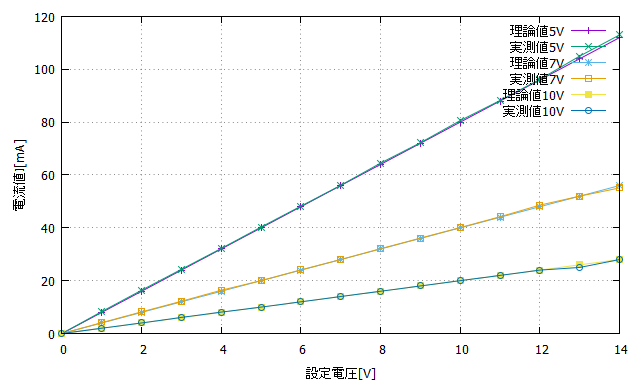
\includegraphics[width=10cm]{02.png}
        \caption{電圧電流特性グラフ}
    \end{center}
\end{figure}

\begin{figure}[H]
    \begin{center}
        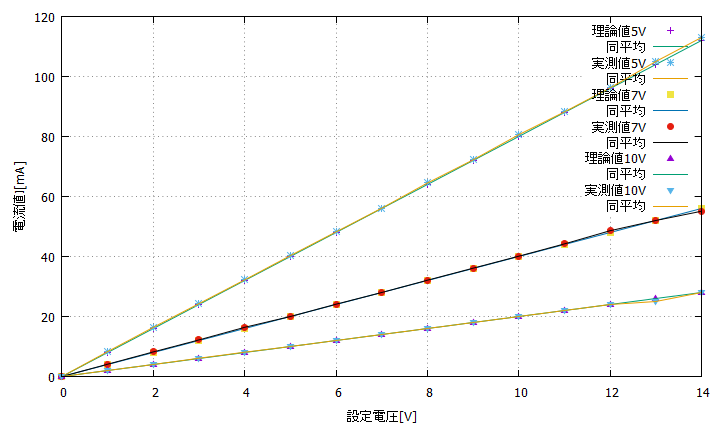
\includegraphics[width=10cm]{03.png}
        \caption{図3 点群プロット及び平均グラフ}
    \end{center}
\end{figure}

\section{考察}
[実験1]抵抗電流特性について、表1より実測値と理論値の誤差は\\
±1mAの範囲に収まっておりほぼ一致しているといえる。
実測値が理論値に一致しているとした場合、\\
5Vの場合では
\begin{equation}
    I[mA]=5[V]/R[kΩ]
\end{equation}
7Vの場合では
\begin{equation}
    I[mA]=7[V]/R[kΩ]
\end{equation}
10Vの場合では
\begin{equation}
    I[mA]=10[V]/R[kΩ]
\end{equation}
であるといえる。よって2章で示された(1)式に一致する。\\
よって電流の大きさと抵抗値の関係にオームの法則が成立することが確認できた。\\

また[実験2]電圧電流特性についても、表2より実測値と理論値の誤差は\\
±1mAの範囲に収まっておりほぼ一致しているといえる。
実測値が理論値に一致しているとした場合、\\
125Ωの場合では
\begin{equation}
    I[mA]=V[V]/125[kΩ]
\end{equation}
250Ωの場合では
\begin{equation}
    I[mA]=V[V]/250[kΩ]
\end{equation}
500Ωの場合では
\begin{equation}
    I[mA]=V[V]/500[kΩ]
\end{equation}
であるといえる。よって2章で示された(1)式に一致する。\\
よって電圧の大きさと電流の大きさの関係にオームの法則が成立することが確認できた。\\

2つの実験から、電流の大きさと抵抗値の関係にオームの法則が\\
電圧の大きさと電流の大きさの関係にオームの法則が成り立つことが分かった。\\
よって、電流の大きさと抵抗値の関係、電圧の大きさの関係にオームの法則が成り立つと言える。\\
また(1)式が確認できたことから、式変形により同様に(2)式、(3)式も同様に成り立つことがわかる。\\
以上のことから2章で示された3つの式は確認され、オームの法則は確認できた。

\section{課題}
今回の[実験1]、[実験2]では、直流電源を使用したため\\
交流の電源を用いた場合、オームの法則が成り立つかどうか確認することができなかった。\\
極性が常に入れ替わる交流電流においてオームの法則が成り立つのか\\
また、どのような挙動をするのか実験をすることは今度の課題である。

\section{感想}
今回は共同実験者に恵まれ、スムーズに実験を行うことができた。\\
計測器の有効桁数の部分で苦戦をしたが、理論値の計算や器具の仕様の記録などを\\
分担で行うことができ、効率の良い実験になった。\\
レポート作成にはVSCodeに整えたLaTeX環境、回路図作成にはKiCad、グラフ作成にはGnuplotを使用した。\\
Texに関しては3年生からこの記法ということで練習を兼ねたが、非常に使いやすく気に入った。\\
課題で述べた交流電流でのオームの法則は、非常に興味があるので調べたい。\\

\end{document}